\chapter{Theoretical overview}
\label{cha:theory}

In this chapter the current best theory of particle physics, the standard model,
is outlined. Outstanding problems are detailed and used to motivate BSM 
physics and, in particular, SUSY. The features of supersymmetric theories are 
outlined and the possible experimental signatures which would enable such a theory to be 
discovered are detailed.

Natural units, Einstein summation convention
and Feynman slash notation are used throughout. Electric charges 
are in units of the charge of the electron.

\section{The standard model}

\label{sec:sm}

The SM of particle physics is a quantum field theory (QFT) whose excitations
correspond to the elementary particles forming all known matter and the mediators of
all known forces~\cite{ftsm}. 

The known matter in the universe is composed of spin-1/2 fermions, summarised 
in Table~\ref{tab:fermions}. These are split into quarks which carry colour charge 
(see Section~\ref{sec:sm-gs}) and leptons which do not. In terms of their
quantum nmbers, each of the three 
generations of quarks and leptons vary only in mass from the other generations. 
The SM contains spinor fields which give rise to these fermions.

The interactions between particles in the universe are mediated by
spin-1 bosons, summarised in Table~\ref{tab:bosons}. 
The gluon and photon are massless while the W and Z bosons are massive. 
The mechanism for determining the masses of these particles, discussed in 
Section~\ref{sec:sm-gs}, gives rise to a further fundamental spin-0 particle, the Higgs boson.
The SM contains vector and scalar fields which give rise to the spin-1 and spin-0
bosons respectively.

The symmetries of the SM determine the properties of the particles and 
their interactions. There are two classes of symmetries:

\begin{itemize}
\item Space-time symmetries corresponding to translations and rotations of the space-time coordinates.
The SM satisfies the Poincar\'{e} group of space-time transformations that define special relativity. 
\item Gauge symmetries corresponding to transformations of the fields within the SM.
\end{itemize}

The mechanism by which the gauge symmetries give rise to the properties and interactions 
of the particles in the SM is detailed in the remainder of this section. 

\begin{table}
  \caption[The fundamental spin-1/2 fermions observed in nature separated into their three generations. 
  Each particle shown also has an antiparticle with opposite charge and identical mass]{The fundamental fermions observed in nature separated into their three generations. 
  Each particle shown also has an antiparticle with opposite charge and identical mass~\cite{pdg}.}
  \label{tab:fermions}
  \begin{tabular}{ccccccc}
  \hline\hline
  &\multicolumn{3}{|c|}{Leptons}& \multicolumn{3}{c}{Quarks} \\
  \cline{2-7}
  Generation & \multicolumn{1}{|c}{Particle} & Mass & \multicolumn{1}{c|}{Electric Charge} & Particle & Mass & Electric Charge \\
  \hline
  \multirow{2}{*}{1} & \Pem & 511 \keV & -1 & \Pqu & 2.3 \MeV & $+\frac{2}{3}$ \\
  & \Pgne & $\sim$0 & 0 & \Pqd & 4.8 \MeV & $-\frac{1}{3}$ \\
  \hline
  \multirow{2}{*}{2} & \Pgmm & 105.7 \MeV & -1 & \Pqc & 1.275 \GeV & $+\frac{2}{3}$ \\
  & \Pgngm & $\sim$0 & 0 & \Pqs & 95 \MeV & $-\frac{1}{3}$ \\
  \hline
  \multirow{3}{*}{2} & \Pgtm & 1.777 \GeV & -1 & \Pqt & 173.2 \GeV & $+\frac{2}{3}$ \\
  & \Pgngt & $\sim$0 & 0 & \Pqb & 4.18 \GeV & $-\frac{1}{3}$ \\
  \end{tabular}
\end{table}

\begin{table}
  \caption[The fundamental spin-1 vector bosons observed in nature and the force which they mediate.]{The fundamental spin-1 vector 
bosons observed in nature and the force which they mediate~\cite{pdg}.}
  \label{tab:bosons}
  \begin{tabular}{lccc}
    \hline\hline
    Force & Particle & Mass & Electric Charge \\
    \hline
    Electromagnetism & \Pgg & 0 & 0 \\
    \hline
    \multirow{2}{*}{Weak} & \PWpm & 80.4 \GeV & $\pm 1$ \\
    \cline{2-4}
    & \PZ & 91.2 \GeV & 0 \\
    \hline
    Strong & g & 0 & 0 \\
  \end{tabular}
\end{table}

\subsection{Gauge symmetries}

The derivation in this section follows that in~\cite{ewk-int}. Consider a Lagrangian containing a fermionic field, $\psi$,

\begin{equation}
\mathcal{L} = \psi(x)^{\dagger} (i\gamma^{\mu}D_{\mu} - m)\psi(x) = \psi(x)^{\dagger} (i\cancel{D} - m)\psi(x),
\end{equation}

where $\psi(x)^{\dagger}$ is the hermitian conjugate of $\psi(x)$, $D_{\mu}$ is the `covariant derivative' and
$\gamma^{\mu}$ are the Dirac matrices. Consider a local gauge symmetry defined by symmetry operator $U(x)$ such that

\begin{align}
\psi(x) &\rightarrow U(x)\psi(x), \\
\psi^{\dagger}(x) &\rightarrow \psi^{\dagger} (x) U^{\dagger} (x).
\end{align}

In the remainder of this section the dependence on x is implicit. In order to ensure gauge invariance, the 
covariant derivative must transform as 

\begin{equation}
\label{equ:cov_deriv}
D_{\mu}\psi \rightarrow U D_{\mu}U^{\dagger} U \psi \rightarrow U \psi.
\end{equation}

This may be achieved by introducing a vector gauge field, $A_\mu$, such that 
$D_{\mu} = \partial_{\mu} + igA_{\mu}$. To satisfy Equation~\ref{equ:cov_deriv},
such that the Lagrangian is gauge invariant, $A_{\mu}$ must transform
under the `adjoint action',

\begin{equation}
A_{\mu} \rightarrow U A_{\mu} U^{\dagger} + \frac{i}{g}(\partial_{\mu}U)U^{\dagger}.
\end{equation}

Having introduced this vector field, a new gauge invariant term may be added to the Lagrangian,

\begin{equation}
\mathcal{L} = \psi^{\dagger} (i\cancel{D} - m)\psi - \frac{1}{4}F^{\mu,\nu}F_{\mu\nu},
\end{equation}

where $F^{\mu\nu}$ is the field strength tensor of the vector field,

\begin{equation}
F_{\mu\nu} = - \frac{1}{g}\left[D_{\mu},D_{\nu}\right] = \partial_{\mu}A_{\nu} - \partial_{\nu} A_{\mu} - g\left[A_{\mu},A_{\nu}\right].
\end{equation}

By writing the fields and covariant derivatives in terms of the generators of the group, $t_{a}$, such
that $A_{\mu} = A^{a}_{\mu} t_{a}$, the field strength tensor can be written as 
\begin{equation}
F^{a}_{\mu\nu}t_{a} = \left(\partial_{\mu}A^{a}_{\nu} - \partial_{\nu} A^{a}_{\mu} - g f_{bc}^{a}A^b_{\mu}A^c_{\nu}\right)t_a,
\end{equation}
where $f_{bc}^{a}$ are the structure constants of the group defined by the 
commutation of the group generators~\cite{wei1963lie}. Non zero structure constants introduce
self interactions of the gauge fields. No gauge invariant term quadratic 
in $A^a_\mu$ (mass term) can be added to the Lagrangian and 
therefore the vector field is massless.

Gauge symmetries of the Lagrangian therefore result in massless vector 
bosons that are `mediators' of the resultant forces. The properties of
the forces depend on the details of the gauge symmetry. 
In the next section, the gauge symmetries
of the SM are discussed. 

\subsection{Gauge symmetries of the standard model}
\label{sec:sm-gs}
The gauge symmetry group of the SM is given by~\cite{ewk-int}:
\begin{equation}
G_{SM} = SU(3)_{c}\otimes SU(2)_{L}\otimes U(1)_{Y}.
\end{equation}

The $SU(3)_c$ gauge symmetry is unbroken and therefore the associated
`strong force' is mediated by a massless vector boson, the gluon.
$SU(3)_c$ is generated by the eight Gell-Mann matrices which give rise to eight colour charges. 
The quarks carry a single colour charge, the gluon is doubly charged and all 
other fundamental particles in the SM are colour singlets. The strong force is short range
as the gluon is self-interacting.  The strong coupling constant, $\alpha_s$, 
reduces with energy (asymptotic freedom)
making calculations non-perturbative~\cite{qcd}. The energy required to separate 
colour singlets of quarks is sufficient to generate additional quark/antiquark pairs
(hadronisation) and therefore quarks are `confined' into colour singlet hadrons
of two (mesons) or three (baryons) quarks. High energy collisions of protons, 
such as those at the LHC, result in the production of highly 
collimated emissions of hadrons (jets) due to the 
liberation of quarks~\cite{salam}.


The gauge symmetry of the electroweak sector of the SM is $SU(2)_L\otimes U(1)_Y$. These symmetries lead
to the electromagnetic and weak forces mediated by the $\gamma$ and W/Z and bosons respectively.

The Lagrangian for this sector may be written as
\begin{equation}
\mathcal{L}_{Ewk} = \mathcal{L}_{gauge} + \mathcal{L}_{fermion} + \mathcal{L}_{Higgs} + \mathcal{L}_{Yuk},
\end{equation}

the terms of which are discussed in this section. The weak force distinguishes
between left and right-handed chiralities and therefore the fermionic fields are split into
$\psi_{L/R} = (1\pm\gamma^5)\psi$. The fermion term may then be written for each of the 
three generations of quarks and leptons as:

\begin{equation}
\mathcal{L}_{fermion} = i \psiL^{\dagger}\cancel{D}\psiL + i \psiR^{\dagger}\cancel{D}\psiR.
\end{equation}

The left-handed fields transform as doublets under the $SU(2)_L$ symmetry
while the right-handed fields are singlets.
For the first generations of quarks and leptons $\psi$ may therefore be written as

\begin{align}
\qquad\qquad\qquad\psiL =\,&{\begin{pmatrix} u_L \\ d_L \end{pmatrix}},\, &{\begin{pmatrix} \nu_{e\,L} \\ e_L \end{pmatrix}},\nonumber\qquad\qquad\qquad\\
\qquad\qquad\qquad\psiR = \,&\,u_R,d_R,\, &\,e_R.\qquad\qquad\qquad
\end{align}

The generators of $SU(2)_L$ are $T^i = \tau^i/2$, where $\tau^i$ are the three Pauli matrices. 
The covariant derivative therefore acts on the left and right-handed components of $\psi$ as

\begin{equation}
D_{\mu} \psiL = (\partial_\mu + igW^i_{\mu}T^i + ig'YB_\mu)\psiL \, D_{\mu} \psiR = (\partial_\mu + ig'YB_\mu)\psiR
\end{equation}

where g and g' are the coupling constants of the $SU(2)_L$ and $U(1)_Y$ groups respectively, 
$W^i$ are the three gauge bosons that couple to the weak isospin, T, and B is the gauge boson
coupling to hypercharge, Y. The hypercharge values are chosen such that the sum of the hypercharge and 
the third component of weak isospin corresponds to the electric charge,
\begin{equation}
\label{equ:charge}
Q = T^{3} + Y.
\end{equation}

For the gauge section of the Lagrangian, the $SU(2)_L$ and U(1) symmetries give rise to two field strength tensors,
\begin{align}
G^i_\mu\nu &= \partial_\mu W^i_\nu - \partial_\nu W^i_\mu - g \epsilon^{ijk}W^j_\mu W^k_\nu,\\
F_\mu\nu &= \partial_\mu B_\nu - \partial_\nu B_\mu.
\end{align}

This leads to

\begin{equation}
\mathcal{L}_{gauge} = -\frac{1}{4}F^{\mu\nu}F_{\mu\nu} - \frac{1}{4}G^{i\mu\nu}G^{i}_{\mu\nu}.
\end{equation}

The Lagrangian invariant under these gauge symmetries, however, does not correspond to the observed universe. No mass terms
can be included for either the gauge bosons or the fermions while maintaining gauge invaraince.
As shown in the remainder of this section, such masses must be introduced via the breaking
of the electroweak gauge symmetry in the Higgs sector of the Lagrangian. 

The Higgs sector of the Lagrangian is given by,

\begin{equation}
\label{equ:higgs-lagrangian}
\mathcal{L}_{Higgs} = (D^{mu}\phi)^{\dagger}(D_{\mu}\phi) - V(\phi)
\end{equation}

where the complex scalar field, $\phi$, is in the spinor representation of $SU(2)_L$. The covariant derivative of $\phi$ is

\begin{equation}
D_{\mu} \phi = (\partial_\mu + igW^i_{\mu}T^i + ig'\frac{1}{2}B_\mu)\phi 
\end{equation}

and the potential, V, is given by

\begin{equation}
V(\phi) =  - \mu^2\phi^{\dagger}\phi + \lambda \left(\phi^{\dagger}\phi\right)^2
\end{equation}

where $\mu^2$ and $\lambda$ are positive constants. The potential is minimised for any $\phi$ satisfying
$\phi^{\dagger}\phi = \frac{\mu^2}{2\lambda} \equiv v^2/2$. While the potential satisfies the 
electroweak gauge symmetry, the minimum will not and may be chosen as

\begin{equation}
\braket{\phi} =  - \frac{1}{\sqrt{2}}\begin{pmatrix} 0 \\ v\end{pmatrix}.
\end{equation}

From Equation~\ref{equ:charge}, the scalar field has zero electric charge and electromagnetism
is an unbroken symmetry. The symmetry group has therefore been broken 
from $SU(2)_L\otimes U(1)_Y \rightarrow U(1)_Q$. Taking the unitary gauge to remove unphysical `Goldstone 
bosons'~\cite{unitGauge}, the scalar field may be expanded around this minima as

\begin{equation}
\label{equ:phiExp}
\phi =  - \frac{1}{\sqrt{2}}\begin{pmatrix} 0 \\ v + H\end{pmatrix}.
\end{equation}

The physical W, Z and $\gamma$ (labelled A) gauge bosons are combinations of the 
bosons defined above,

\begin{equation}
W^{\pm} = \frac{1}{\sqrt{2}} (W^1_\mu \mp i W^2_\mu), \begin{pmatrix} Z_\mu \\ A_\mu\end{pmatrix} = \begin{pmatrix} \cos(\theta_W) & -\sin(\theta_W) \\ \sin(\theta_W) & \cos(\theta_W)\end{pmatrix} \begin{pmatrix} W^3_\mu \\ B_\mu\end{pmatrix}
\end{equation}

where $\theta_W \equiv \text{atan}(g'/g)$ is the weak mixing angle. From Equation~\ref{equ:phiExp} and
the first term of Equation~\ref{equ:higgs-lagrangian}, the masses may be identified as

\begin{equation}
M_W^\pm = \frac{1}{2}gv, M_Z = \frac{gv}{2cos\theta_W}, M_A = 0
\end{equation}

The masses of the fermions are derived from the Yukawa term in the Lagrangian, 
\begin{equation}
\mathcal{L}_{Yuk} = - \frac{1}{\sqrt(2)}(v + H)(f_{mn} e_L^{\dagger}e_R + h_{mn} d_{Lm}^{\dagger}d'_{Rn} + k_{mn} u_{Lm}^{\dagger}u_{Rn}) + \text{hermitian conjugate}
\end{equation}

where $f_{mn}$, $h_{mn}$ and $k_{mn}$ are the Yukawa coupling matrices between the different generations. These may be diagonalised via unitary transformations
to generate mass terms for the quarks and leptons. The neutrino is massless in the SM as there is no right-handed component.
This contradicts the observation of oscillations between neutrino flavours~\cite{neutOsc},
however, extensions which predict non-zero neutrino masses are possible~\cite{neutM}. 

The same unitary transformations also introduce mixing between quark generations from the 
terms including covariant derivatives in the Lagrangian. The mixings are summarised in the 
CKM matrix and occur as no basis of mass eigenstates is simultaneously diagonal for 
up and down type quarks~\cite{CKM}. Flavour changing
interactions between quarks are mediated by the $W^{\pm}$ boson while interactions via 
the Z and $\gamma$ bosons are flavour preserving. There are no flavour changing interactions
predicted for the leptons.

\section{Physics beyond the standard model}

The SM describes the properties and interactions between all known particles. These properties 
have been measured and the predictions of the SM verified in a multitude
of experiments. However, the theory cannot be complete 
as there remain fundamental problems which the standard model does not resolve.
Several of the largest such problems are described below.

On a theoretical level, a renormalisable theory of gravity cannot be included within 
the SM~\cite{gravRenorm}. While negligible at electroweak energy
scales, quantum gravitational effects become increasingly important as
energies approach the planck scale, $M_{\text{planck}} \sim 10^{18} \GeV$. 

Measurements from cosmology and astrophysics have highlighted several areas
the SM fails to adequately describe Nature. The vacuum energy density 
of the universe (`cosmological constant'), $\Lambda$, 
may be expected to be approximated by $M^4_{\text{planck}}$ by dimensional 
arguments. However, cosmological measurements of $\Lambda$ imply 
$\Lambda/M_{\text{planck}}^4 \sim 10^{-120}$~\cite{cosConst}. This discrepancy
is related to the failure to include gravity in a quantum field theory.

Astrophysical observations~\cite{WIMP} imply the existence 
of a weakly-interacting particle (WIMP) that forms the majority of the matter 
within the universe. The SM has no viable candidates for 
this particle. In addition, the matter-antimatter asymmetry observed in the universe requires 
charge-parity violating processes far in excess of those occurring in the SM.

The discovery of the Higgs boson at $m_{h}\sim125\,\GeV$ raises the `hierarchy problem'. In QFT, 
the corrections to $m_h$ are related to the heaviest particle in the theory and therefore
one may expect $m_h \sim M_{\text{planck}}$. In addition, quantum corrections from SM particles
require fine-tuning in the SM to stabilise $m_h$ (the `technical hierarchy problem', see Section~\ref{sec:natSUSY}).

These problems form the motivation for the existence of a BSM physics model that
can resolve some or all of the outstanding issues in the SM. SUSY is a particularly
well motivated BSM theory that can resolve the hierarchy problem, provide a DM candidate
and include a quantum theory of gravity.

\section{Supersymmetry}

There are many possibilities for extending the SM, 
including new particles/interactions, new (internal) gauge symmetries, 
extra spacial dimensions and/or new space-time (external) symmetries. SUSY is 
an external symmetry that relates fermions and bosons by extending the Poincar\'{e} algebra~\cite{SUSYC}. 
The Coleman-Mandula theorem shows that any such extension through new bosonic generators (such as those responsible for Lorentz 
transformations and translations) forbids non-zero scattering amplitudes~\cite{Coleman}. 
Supersymmetry therefore introduces fermionic generators, Q, such that (heuristically),

\begin{equation}
Q\ket{\text{Boson}} \sim \ket{\text{Fermion}} \quad Q\ket{\text{Fermion}} \sim \ket{\text{Boson}}.
\end{equation}

Particles connected by the SUSY generator are in `supermultiplets'. This generator commutes with all gauge symmetries 
of the SM and so particles within each supermultiplet have identical electric, weak isospin and colour charges.
In addition, the SUSY generator commutes with the mass operator, implying 
particles within each supermultiplet have identical masses. The supersymmetric partners of the 
known SM particles, `sparticles', have not been observed and therefore SUSY must be a broken symmetry.

\subsection{The minimally supersymmetric standard model}

The minimally supersymmetric standard model (MSSM) is the simplest supersymmetric extension of the SM~\cite{SUSYP}.
The fermions in the SM are `chiral' (left and right-handed pieces transform differently)
with two fermionic degrees of freedom per helicity state. The number of bosonic and fermionic degrees 
of freedom must be equivalent in each supermultiplet and therefore the simplest supermultiplet
is the chiral supermultiplet containing the fermion and two real scalar fields.

The gauge bosons in the SM (before electroweak SUSY breaking) are massless spin-1 vector bosons
and therefore have two bosonic degrees of freedom (one per helicity state) and
can be included in a `gauge' supermultiplet with a spin-1/2 fermionic partner (`gaugino').

The SM Higgs does not reside in a single chiral supermultiplet as this introduces
a gauge anomaly into the theory~\cite{SUSYP}. This anomaly may be avoided by including two Higgs 
chiral supermultiplets with opposite hypercharge. The SM Higgs is a linear combination of the neutral components 
of these supermultiplets.

\begin{table}[!h]
  \centering
  \caption{Chiral supermultiplets in the MSSM~\cite{SUSYP}}
  \label{tab:chiral}
  \begin{tabular}
    {ccc}
    \hline\hline
    Name& spin-0 & spin-1/2 \\
    \hline
    \multirow{3}{*}{squarks, quarks (3 families) }& ($\tilde{u}_L\,\tilde{d}_L$) & ($u_L\,d_L$) \\
    & ($\tilde{u}^{*}_R$) & ($u_R^{\dagger}$) \\
    & ($\tilde{d}^{*}_R$) & ($d_R^{\dagger}$) \\
    \hline
    \multirow{2}{*}{sleptons, leptons (3 families) }& ($\tilde{\nu}\,\tilde{e}_L$) & ($\nu_L\,e_L$) \\
    & ($\tilde{e}^{*}_R$) & ($e_R^{\dagger}$) \\
    \hline
    \multirow{2}{*}{Higgs, higgsinos}& ($H_u^{+}\,H_u^{0}$) &  ($\tilde{H}_u^{+}\,\tilde{H}_u^{0}$) \\
    & ($H_d^{0}\,H_d^{-}$) &  ($\tilde{H}_d^{0}\,\tilde{H}_d^{-}$) \\
  \end{tabular}
\end{table}

\begin{table}[!h]
  \centering
  \caption{Gauge supermultiplets in the MSSM~\cite{SUSYP}}
  \label{tab:vector}
  \begin{tabular}
    {ccc}
    \hline\hline
    Name& spin-0 & spin-1/2 \\
    \hline
    gluino, gluon & $\tilde{g}$ & g \\
    winos, W bosons & $\tilde{W}^{\pm}\,\tilde{W}^0$ & $W^{\pm}\,W^{0}$ \\
    bino, B boson & $\tilde{B}^0$ & g \\
  \end{tabular}
\end{table}

The particle content of the MSSM (before symmetry breaking) 
is summarised in Table~\ref{tab:chiral} for the chiral supermultiplets
and Table~\ref{tab:vector} for the gauge supermultiplets. The neutral higgs and electroweak 
gaugino sectors combine to form mass eigenstates labelled `neutralinos' 
(\chiz), while the charged higgs and electroweak gaugino sectors combine
to form `charginos' (\chip). Gravity may also be included in the theory
by adding a spin-2 graviton and a spin-3/2 superparticle
called the gravitino~\cite{SUSYP}. 

The mass scale of the sparticles is dependent on the mechanism of SUSY breaking.
As discussed below, naturalness arguments motivate the lightest sparticle masses 
at the \TeV~scale.

\subsection{Natural supersymmetry}
\label{sec:natSUSY}
In the SM, the Higgs mechanism requires couplings to each fermion, f, of the form $-\lambda_{f}f^{\dagger}f\phi$. If BSM physics
is expected to alter the high energy behaviour of the theory at a scale $\LUV$, the quantum corrections 
to the Higgs boson mass, $\delta m^2_{H}$, will be 

\begin{equation}
\Delta m^2_H =  \frac{|\lambda_f|^2}{8\pi^2}\left[-\Lambda^2_{\text{UV}}\right] + \mathcal{O}\log(\LUV)
\end{equation}

which is quadratically divergent~\cite{HMSSM}. The correction is proportional to the size of the coupling of the Higgs to the fermion 
and is therefore largest for the top quark in the SM. Assuming the cut-off scale is at $M_{\text{planck}}$, the quantum 
corrections must be fine-tuned to $\sim 30$ orders of magnitude to predict the observed Higgs mass. 

In a BSM theory containing complex scalars, s, the Lagrangian will gain a term $-\lambda_{s}|\phi|^2|s|^2$.
Assuming, for simplicity, each component of the complex scalar has mass $m_s$, the correction to the Higgs mass will be

\begin{equation}
\label{equ:corrHiggsSusy}
\Delta m^2_H =  \frac{\lambda_s}{8\pi^2}\left[-\Lambda^2_{\text{UV}}\right] + \mathcal{O}\log(\LUV),
\end{equation}

If SUSY is a symmetry of nature, each fermion can be related to a complex scalar such that $|\lambda_f|^2 = -\lambda_s$ 
and the quadratic divergence is naturally cancelled. In unbroken SUSY, logarithmic divergences also vanish~\cite{HMSSM}. 
Experimental observations imply the sparticle masses cannot be equal to their SM partners and
therefore an additional SUSY breaking term is required in the Lagrangian. This must be a `soft' breaking,
such that $\lambda_f^2 = -\lambda_s$ still holds to cancel the quadratic divergence.
To avoid fine tuning of the logarithmic divergence, the lightest sparticles should have 
masses around the $\TeV$ scale. The LHC provides the first experimental probe of this energy scale.

\subsection{R-parity}

The general MSSM `super potential' contains terms which violate baryon number, B, and lepton number, 
L. Such terms lead to predictions of proton decay in the order of seconds. 
The proton lifetime is constrained experimentally to $> 10^{34}$ years~\cite{protonDecay},
therefore, to forbid such a process, an extra symmetry called `R-parity' is defined as,
\begin{equation}
R \equiv (-1)^{3(B-L)+2S} = 
\begin{cases}
+ 1\quad \text{SM particles}\\
- 1\quad \text{superpartners}
\end{cases},
\end{equation}
where S is the spin~\cite{SUSYP}. R-parity has several physical implications including a stable lightest supersymmetric 
particle (LSP). This particle must be electrically and colour-neutral from cosmological constraints.
Typically, it is taken to be the lightest neutralino in the MSSM and is an ideal WIMP candidate for DM. 
In addition, R parity requires that superpartners be
formed in pairs in collisions and that each superpartner decays to another superpartner
in a chain that must end with the LSP. The LSP does not interact with any detector and therefore
such collisions will produce signatures containing significant momentum imbalance.

\subsection{Experimental SUSY signatures at the LHC}

The LHC provides proton-proton collisions at $\sqrt{s} = 13\,\TeV$. The sparticles have identical charges under 
the symmetries of the SM and, therefore, in a generic (natural) MSSM model 
coloured sparticles may be expected to have the highest production 
cross-section~\cite{susyprod}. Assuming R-parity, these sparticles can be produced through:

\begin{itemize}
\item quark-antiquark scattering or gluon fusion to produce a gluino or squark pair
\item quark and gluon scattering to produce a squark and gluino
\item quark-quark scattering to produce a squark pair.
\end{itemize}

Each of the sparticles will decay in a chain to the LSP. In the decay, 
coloured SM particles are produced which will hadronise into jets.
The signature produced by such processes will therefore be significant hadronic activity in 
the form of jets as well as momentum imbalance from the LSP. The energy in
the final state and the momentum carried by the LSP are dependent on the masses
of the sparticles.

The top makes the largest contribution to the Higgs boson mass divergence. In natural SUSY, 
the lightest sparticle is expected, therefore, to be the partner of the top. This leads to a signature
of multiple top quarks in the final state. As discussed in Section~\ref{sec:ewk-background-intro}, top quarks
decay primarily to a b quark and W boson. The sparticles produced at the LHC 
may therefore be expected to lead to a final state containing multiple b quarks.

The SM contains processes which produces events with similar signatures to 
those of hadronic SUSY described above. These are described fully in Section~\ref{sec:ewk-background-intro},
and, in order to be sensitive to SUSY signals, such background processes must be mitigated 
and any residual background contributions measured. The search described in this thesis relies on several
techniques to mitigate and measure background processes as described in Chapters~\ref{cha:alphat} and~\ref{cha:backgroundPrediction}
respectively.

\subsection{Simplified models}

The MSSM contains up to 120 free parameters that affect the production and decay modes of the sparticles.
It is therefore not possible to interpret the results of searches for SUSY in the full MSSM. 
In previous searches for SUSY, the constrained MSSM (the CMSSM), which leaves five free parameters, was 
used to interpret the results~\cite{CMSSM}. However, while parametrically simple, the decay chains of sparticles 
in the CMSSM are complicated, making such interpretations model-dependent. 

To evaluate model-independent reach in terms of gluino and squark masses, searches are interpreted using 
simplified models that are defined by a fixed set of production and decay modes.
Simplified models are effective models where the majority of the particle content in the theory 
are decoupled at high masses. Each of the simplified models considered in this thesis involves
the direct pair production of only one sparticle type, which then decays directly to the LSP~\cite{SMS}.

The T2 simplified models are simplified versions of squark-antisquark production. Each squark undergoes
a two-body decay to a quark and the LSP. In this thesis, direct bottom squark production followed
by decay to bottom quark and LSP as well as direct top squark production followed by decay to top
quark and LSP are considered.

The T1 simplified models are a simplified versions of gluino pair production. Each gluino undergoes a three-body 
decay to a quark-antiquark pair and the LSP. In this thesis, decays to top-antitop as well as bottom-antibottom
pairs are considered. As the three body decay proceeds via the virtual squark, these models 
are referred to as gluino-mediated squark production.

\begin{figure}[h!]
  \begin{center}
    \subfloat[Gluino mediated bottom squark production]{
      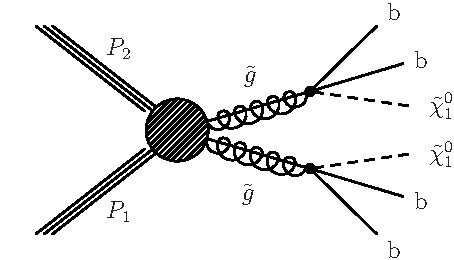
\includegraphics[width=0.4\textwidth]{Figures/theory/T1bbbb_feyn}
      \label{fig:T1bbbb_feyn}
    } ~~
    \subfloat[Glunio mediated top squark production]{
      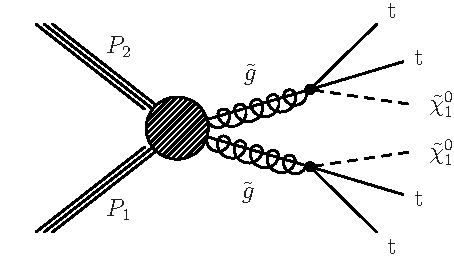
\includegraphics[width=0.4\textwidth]{Figures/theory/T1tttt_feyn}
      \label{fig:T1tttt_feyn}
    } \\
    \subfloat[Direct bottom squark production]{
      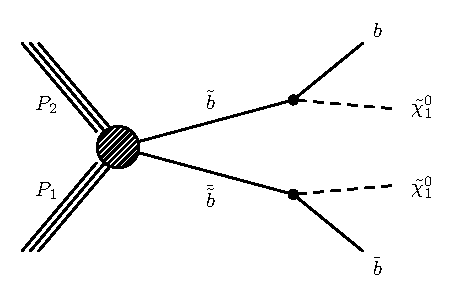
\includegraphics[width=0.4\textwidth]{Figures/theory/T2bb_feyn}
      \label{fig:T2bb_feyn}
    } ~~
    \subfloat[Direct top squark production]{
      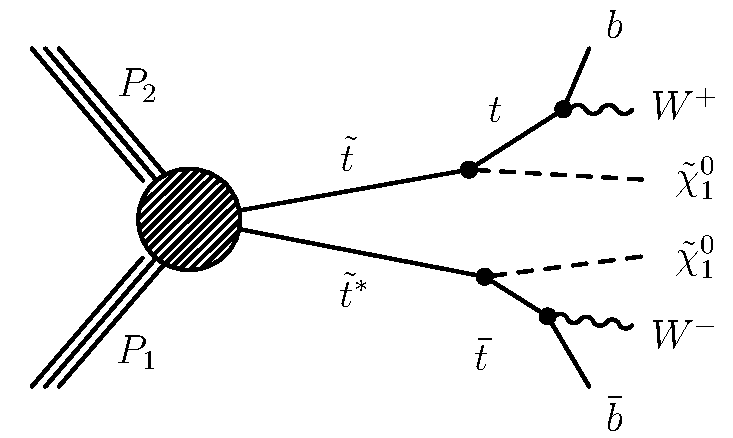
\includegraphics[width=0.4\textwidth]{Figures/theory/T2tt_feyn}
      \label{fig:T2tt_feyn}
    } 
    \caption{
      Graphical representation of the production and decay of supersymmetric particles 
      for the simplified models considered in this thesis~\cite{SMS}.
    }
    \label{fig:simplified-models-feyn}
  \end{center}
\end{figure}

Figure~\ref{fig:simplified-models-feyn} displays the decay chains for the models considered in this thesis. 
In the simplified models, the masses of the heavy sparticle and of the LSP are free parameters.
The topology of the model is crucial in determining the reach of experimental searches. 
In cases where the mass splitting is large, the final state typically contains significant
momentum imbalance and hadronic energy. If the mass splitting is small, (`compressed' models),
the momentum imbalance and hadronic energy are suppressed. Additional phenomena, such as initial/final state radiation (ISR/FSR), 
where one or more incoming/outgoing partons radiates a jet, may be required for sensitivity to such models.

The simplified models may be used to approximate the impact of searches on a complete theory 
by determining the relevant simplified topologies contained in the full theory. The impact
of searches for many different types of signatures may be combined using programs 
such as FastLim~\cite{Fastlim}.

At the end of the 7 and 8~\TeV~centre of mass energy runs of the LHC, the furthest
gluino mass excluded (see Section~\ref{sec:limits}) for the gluino mediated top and bottom 
squark production simplified models was $\sim 1300\,\GeV$ while for direct top and 
bottom squark production, the highest squark mass excluded was $\sim 700\,\GeV$~\cite{limits8}. 
As the centre of mass energy increases to $13\,\TeV$, the production cross section for coloured sparticles
at the~\TeV~scale jumps by more than an order of magnitude~\cite{snowmass}, presenting
an ideal opportunity for the discovery of $\TeV$ scale natural SUSY.




